%----------------------------------------------------------------------------
\chapter{A multiprocesszoros OpenCL környezet} \label{sec:opencl}
%----------------------------------------------------------------------------

\section{OpenCL architektúrája}
	Az Open Computing Language (OpenCL) keretrendszer \cite{opencl}
	általános modellt, magas szintű programozási interfészt és hardware
	absztrakciót nyújt a fejlesztőknek adat-, vagy feladat párhuzamos számítások gyorsítására különböző
	számítóegységen (CPU, GPU, FPGA, DSP, \ldots).
	A hardvergyártók implementálják az OpenCL szabványt, ami által saját platformot
	hoznak létre. Egy ilyen platformon belüli eszközök alatt főként GPU-kat, de
	CPU-kat és FPGA-t \ldots is értünk.
	OpenCL keretrendszerben történő programozás során két programot kell írnunk.
	Az egyik a kernel, ami az eszközön futtatott szálra fog leképeződni.
	A másik a gazda processzoron (host-on) futó host-program, ami elvégzi az I/O műveleteket,
	a probléma összeállítását, a memória allokálást, az argumentumok beállítását
	illetve a kernel meghívását az eszközön.
	A kernel futása végeztével a host-program kiolvassa az eszközből
	a kívánt eredményt.
	
	\begin{figure}[!ht]
		\centering
		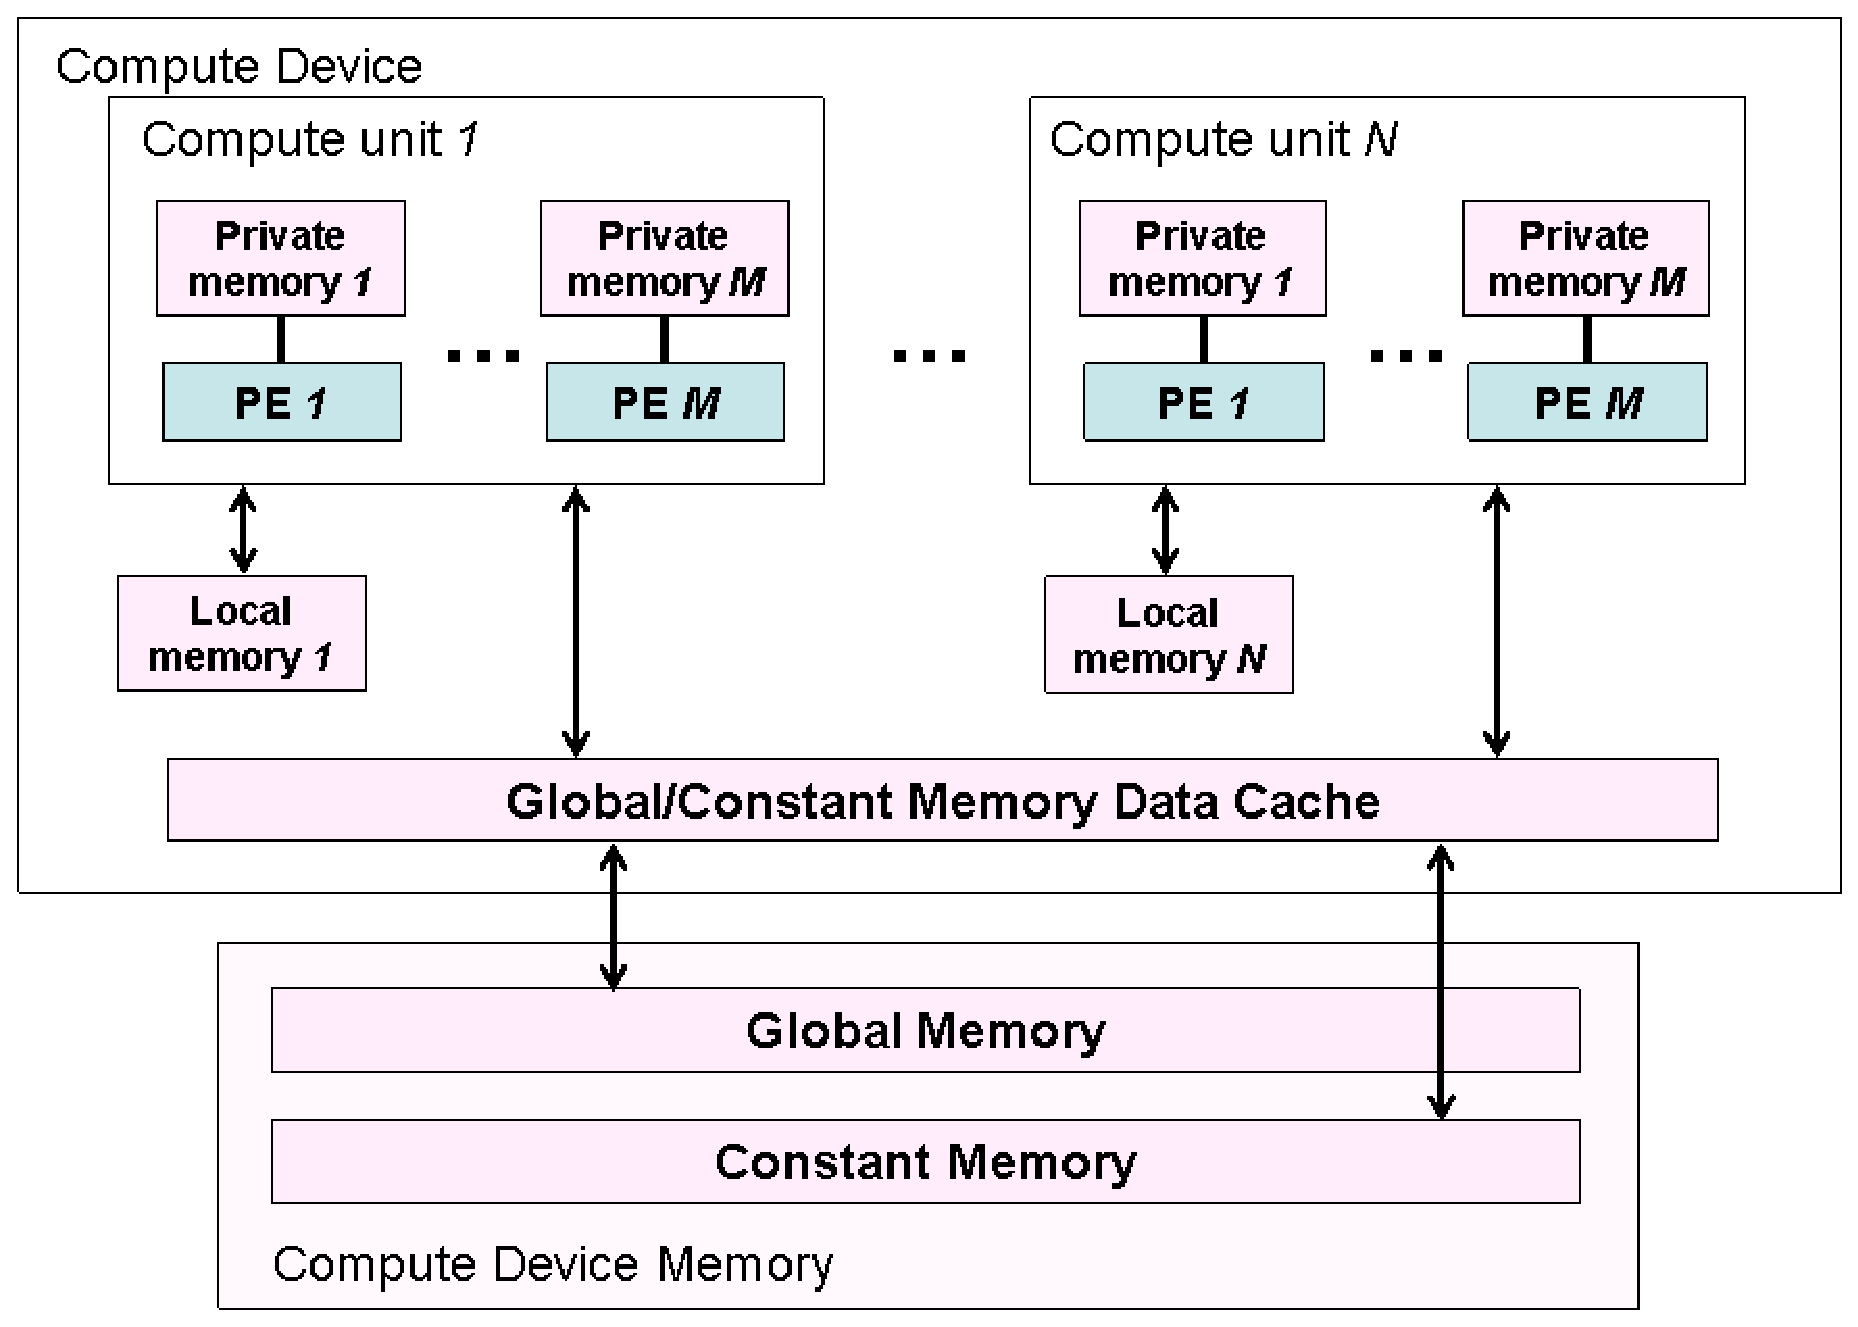
\includegraphics[width=0.6\columnwidth]{figures/eps/device.eps}
		\caption[OpenCL device architektúra]{OpenCL device architektúra (forrás: \cite{opencl})} 
		\label{fig:device} 
	\end{figure}
	Az eszközök multiprocesszoros architektúrával és ezek kiszolgálására képes
	memória architektúrával rendelkeznek, amit a \ref{fig:device} ábra vázol.
	Egy eszköz több compute unit-ot (processzor-magot) tartalmaz.
	Az OpenCL négy memória szintet különböztet meg, amikre a
	következőképpen hivatkozik:
	\begin{itemize}
		\item \emph{Regiszterek:} Private memory,
		\item \emph{Chipen belüli memória (cache):} Local memory,
		\item \emph{Chipen kívüli memória:} Global memory és Constant Memory.
	\end{itemize}
	A regiszterek és lokális memória kis méretűnek és gyors elérésűnek mondható, míg
	a globális memória nagynak, de lassú elérésűnek.
	A memóriákra megkötésként szolgál, hogy ki allokálhat, írhat és olvashat
	belőle. A \ref{table:mem}. táblázatban látható ezen jogosultságok.
	\begin{table}[!h]
	%\renewcommand{\arraystretch}{1.3}
	% if using array.sty, it might be a good idea to tweak the value of
	% \extrarowheight as needed to properly center the text within the cells
	\centering
	% Some packages, such as MDW tools, offer better commands for making tables
	% than the plain LaTeX2e tabular which is used here.
	\begin{tabular}{l|l|l|l|l}
			 & Global memory & Constant mem. & Local mem. & Private mem.\\ \hline
		Host & Dinamikusan R/W & Din. R/W & Din. R/W & \\
		Kernel & R/W & Statikusan R & Satik. R/W & Statik. R/W\\
		Sebesség & Lassú & Gyors & Gyors & Regiszter\\
		Méret & $1$ Gbyte $<$ & $\sim64$ Kbyte& $\sim16$ Kbyte & $<1$ Kbyte
	\end{tabular}
	
	\caption{OpenCL memória szintek}
	\label{table:mem}
	\end{table}
	
	Ahhoz, hogy a rendszerben rejlő teljesítményt kihozzuk három fontos kérdést
	kell a szimulátor magjának implementálásakor megválaszolnunk:
	\begin{itemize}
		\item \emph{Mennyit?} Tisztában kell lennünk az aktuális
		memória fogyasztással és a szükséges memóriamérettel.
		\item \emph{Honnan-hova?} Fontos, hogy a lehető legközelebb legyen az adat
		a processzor-maghoz.
		\item \emph{Mikor?} Mivel a memória művelet alatt a futtatott kernel nem
		dolgozik, így átadja a helyét egy másiknak. (Ez Direct Memory Access (DMA)
		blokk létezése alatt igaz). Ennek a megfelelő szinkronizációjával nagyobb
		kihasználtság érhető el (load balance).
	\end{itemize}
	
	
\section{OpenCL programozási modell}
	
	A programozási modell középpontjában a kontextus áll, ami az OpenCL
	osztálydiagramján (\ref{fig:class}. ábra) figyelhető meg.
	A futtatáshoz szükséges, hogy a kontextushoz platformot, majd azon belül
	eszközt, az eszközhöz programot (kernelt) és memóriát rendeljünk.
	\begin{figure}[!ht]
		\centering
		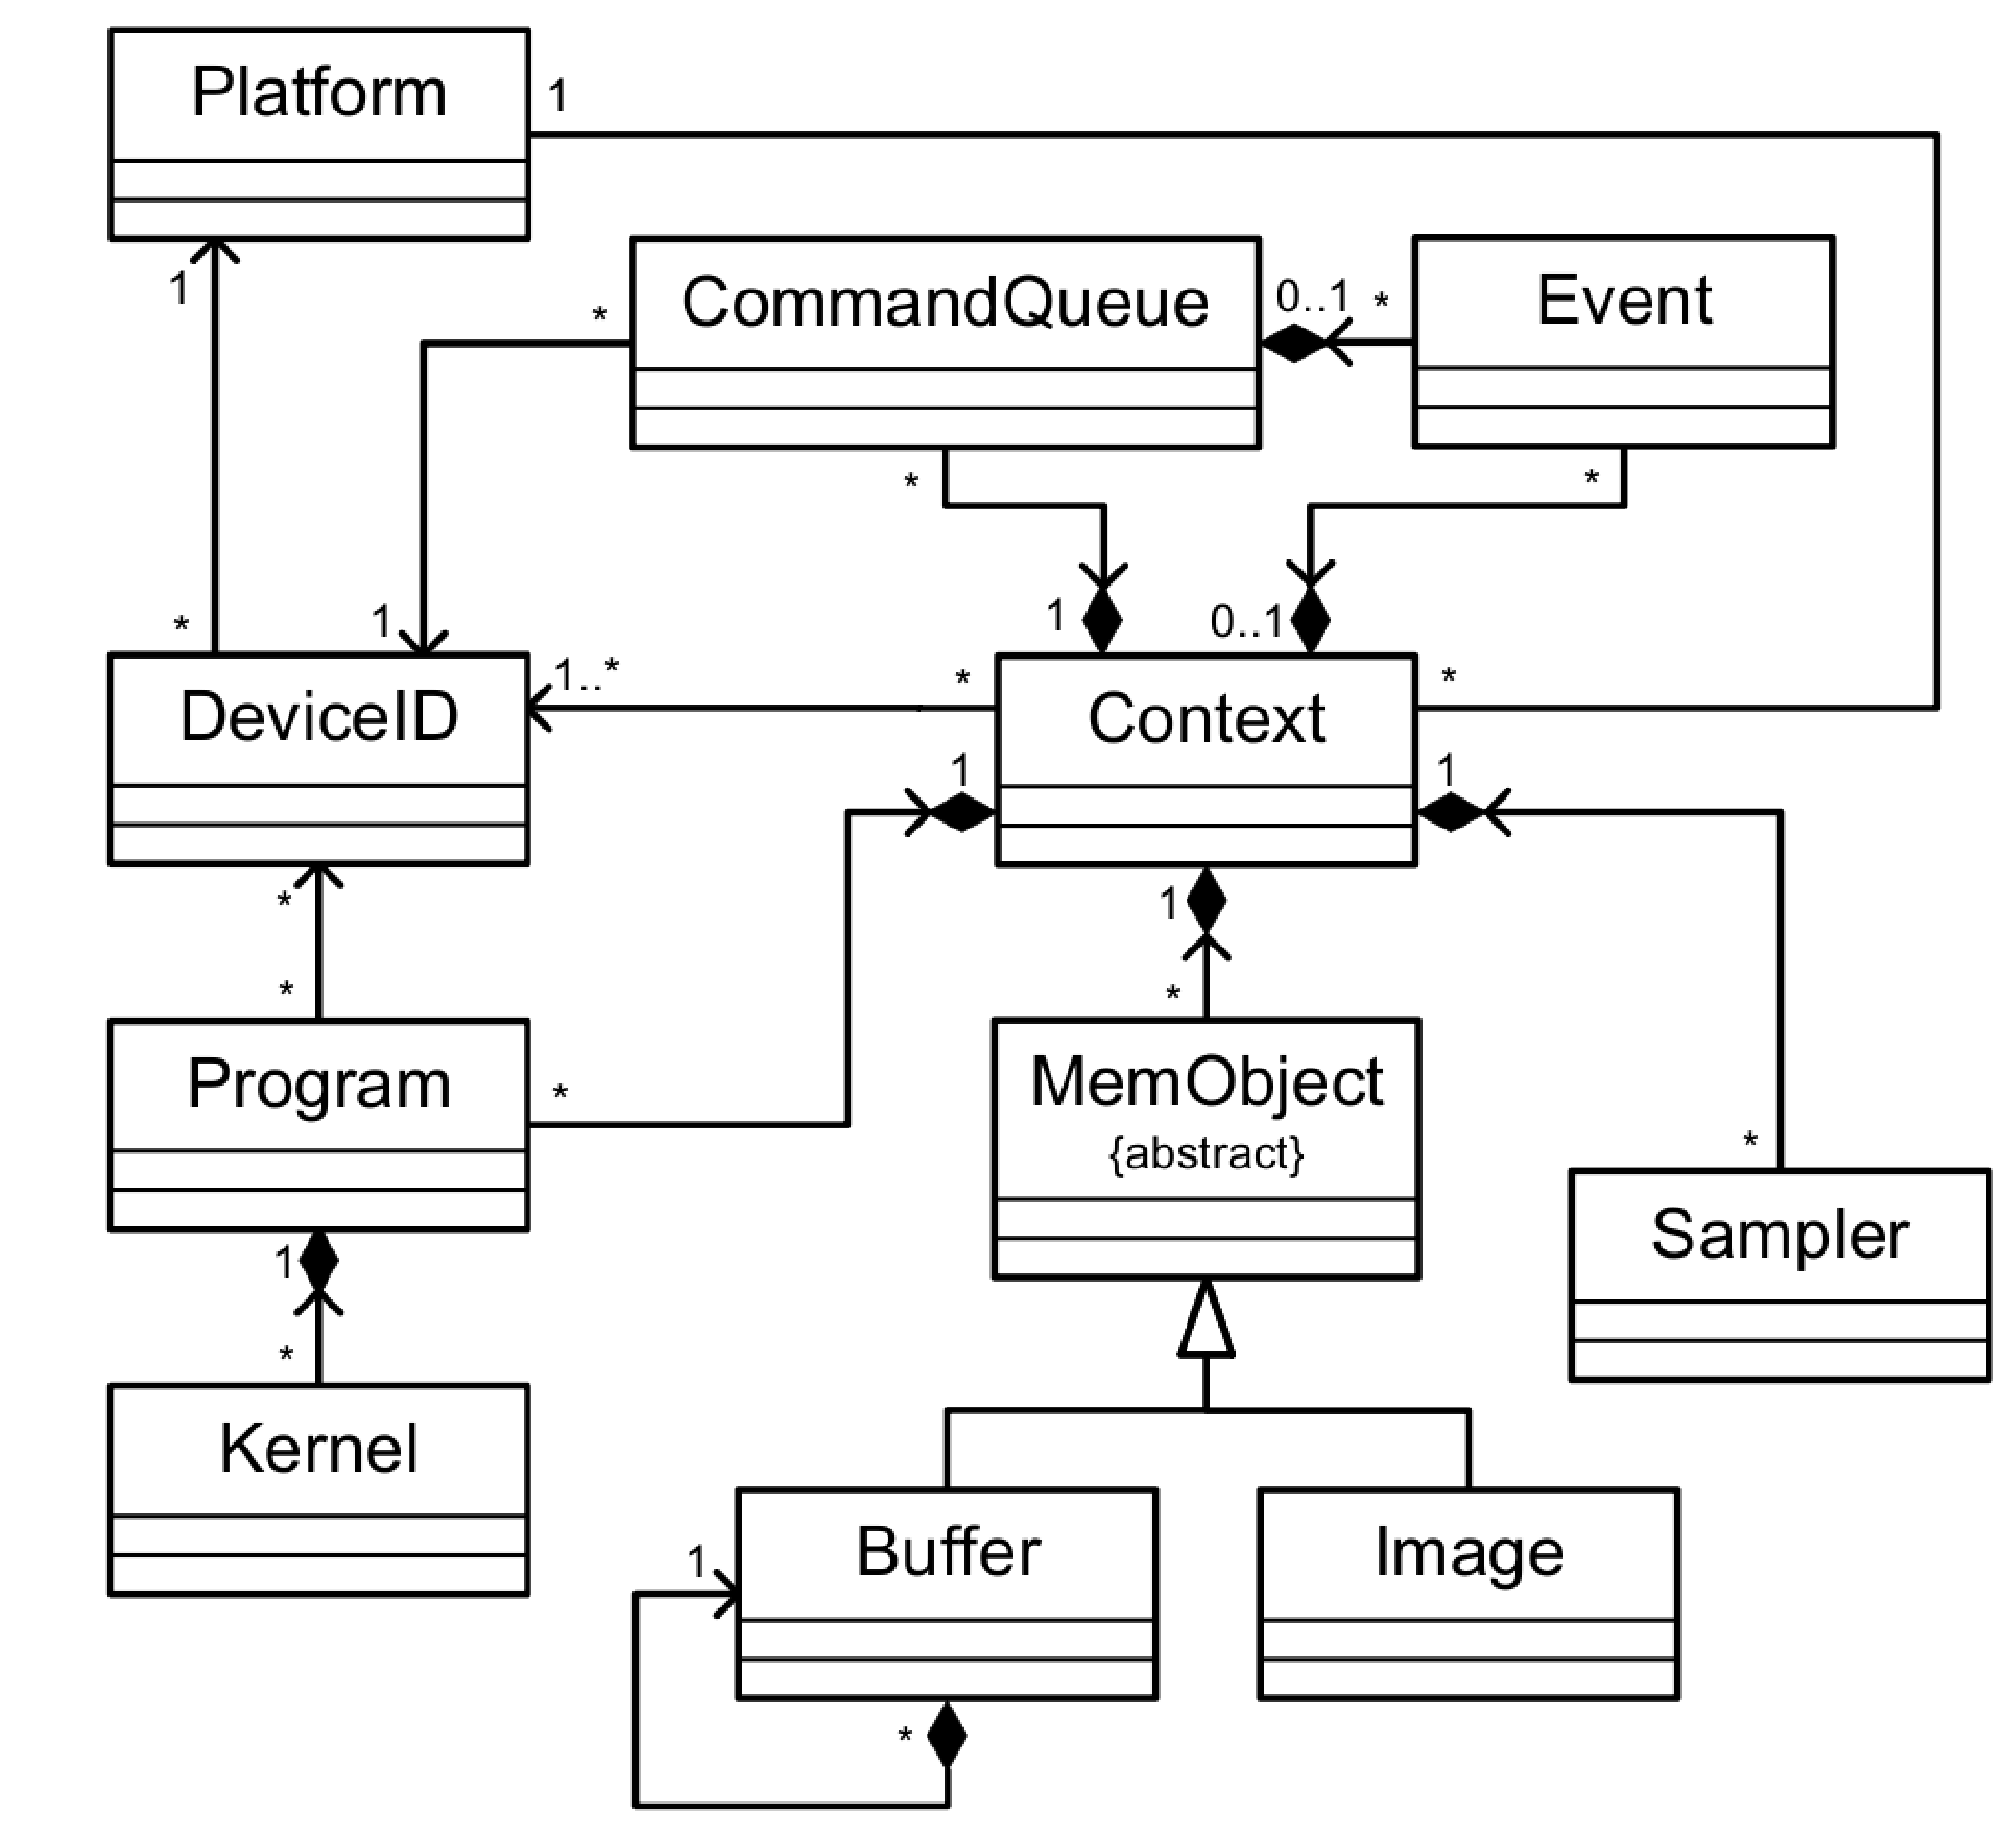
\includegraphics[width=0.6\columnwidth]{figures/eps/context.eps}
		\caption[OpenCL context osztálydiagrammja]{OpenCL context osztálydiagrammja (forrás: \cite{opencl})} 
		\label{fig:class} 
	\end{figure}
	Figyelembe kell vennünk azt a megkötést, hogy csak az egy platformon belüli
	eszközök programozhatóak heterogén módon. Például: Intel platform esetén
	lehetséges CPU-t, processzorkártyát és Intel-es GPU-t programozni.
	
	A programozással megoldandó problémát kétféleképpen lehetséges a feldolgozó
	egységekhez (work-item) avagy processzorokhoz rendelni:
	adat parallel módon vagy taszk parallel módon.
	
	Adat parallel módon (\ref{fig:data_parallel} ábra) a feldolgozandó adat egy
	részéhez rendelünk egy feldolgozó egységet. Fontos figyelembe venni az eszköz korlátos
	számú feldolgozó egységének számát. Ha nem elég a 
        rendelkezésre álló feldolgozó egység, akkor a
	feladat megfelelő particionálásával lehetséges az aktuális
        konfiguráció erőforrásaihoz illeszkedni.
	
	Taszk parallel módot (\ref{fig:task_parallel} ábra) olyan esetben célszerű
	használna, ha a bemenet dinamikus mérete a futási időben
        rendkívül változik
	illetve a végrehajtandó feladat lazán függenek össze.
	
	\begin{figure*}[!ht]
		\centering
		\subfloat[Adat parallel]{
			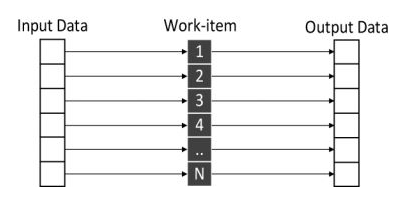
\includegraphics[width=0.45\columnwidth]{figures/eps/data.eps}%
			\label{fig:data_parallel}
		}
		\hfil
		\subfloat[Taszk parallel]{
			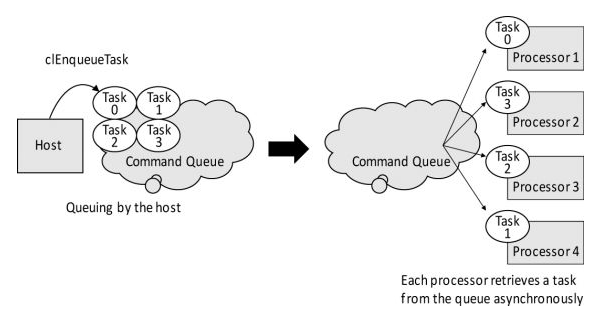
\includegraphics[width=0.45\columnwidth]{figures/eps/task.eps}%
			\label{fig:task_parallel}
		}
		\caption{Feladat hozzárendelése work-item-hez (processzorhoz)}
		\label{fig:parallel}
	\end{figure*}
	A processzor-magok megfelelő kihasználtságának elérése végett több ezer
	work-item virtuálisan osztozik rajta.
	Továbbá ezen work-item-eket work-group-okba rendezzük.
	
	A work-itemeket jelen pillanatban az OpenCL specifikációja
        \cite{opencl} szerint max. 3 dimenziós
	work-group-ba tudjuk rendezni. A következő \ref{fig:ndrange}. ábrán egy 2D-s példát láthatunk egy work-item indexének a globális
	és lokális megfelelőjére.
	
	\begin{figure}[!h]
		\centering
		\includegraphics[width=0.9\columnwidth]{figures/eps/ndrange.eps}
		\caption[2D-s work-item-ek work-group-ba rendezése és indexelése]{2D-s work-item-ek work-group-ba rendezése és indexelése
		(forrás: \cite{opencl})}
		\label{fig:ndrange} 
	\end{figure}

	A work-group-okba rendezés a lokális memória jogosultsága miatt érdekes.
	Konkrétan az egy work-group-ba tartozó összes work-item azonos lokális memórián
	osztozik.
	Ennek a következménye az, hogy adat parallel módú feldolgozás esetén
	az egymásra ható adatokhoz tartozó work-item-eket egy work groupba kell
	rendelnünk.
	Ha ez nem lehetséges, akkor a globális memóriához kell fordulnunk.
	A globális memória avagy a bank szervezésű külső (off-chip) memóriák
	hozzáférési ideje relatíve nagy így ezek használatát lehetőleg el kell kerülni
	és a programozónak kell ``cachelni" a lokális memóriába.
	
	Mivel a work-item-ek konkurensen hajtódnak végre, így az általuk közösen elérhető memóriákra
	(globális, lokális) nézve versenyhelyzetben vannak.
	Az OpenCL ezt a problémát a laza memóriamodell használatával oldja meg. Az alkalmazott
	szinkronizáció egy korlátot tesz a programban, amit csak akkor léphet át, ha az összes többi
	work-item az azonos work-group-ban ezt a korlátot már elérte. Erre a \texttt{barrier(FLAG)}
	függvényhívás szolgál. Fontos megjegyezni, hogy ez a szinkronizáció csak egy adott
	work-group-on belül történik, a work-group-ok közötti szinkronizációra nincs lehetőség. 
	
	\begin{center}
	Összefoglalva: nagy hangsúlyt kell a memóriaszervezésre fordítani, hogy a
	processzormagok megfelelően legyenek az adatokkal táplálva.
	\end{center}


\section{Futási környezet bemutatása}
	A következő eszközök teljesítményét vizsgálom:
	\begin{itemize}
		\item A laptopomban található \textbf{nVidia GTC 330m} notebook-videokártya,
		\item Asztali PC-ben található \textbf{Intel Xeon E5-1620} processzor,
 		\item Asztali PC-ben található \textbf{Intel Xeon Phi} co-processzor kártya \cite{phi,mic},
 		\item Asztali PC-ben található  \textbf{nVidia GTX 590} videokártya.
	\end{itemize}
	Ezen eszközök legjelentősebb paraméterei a \ref{table:envs} táblázat tartalmazza.
	
	\begin{table}[!h]
	%\renewcommand{\arraystretch}{1.3}
	% if using array.sty, it might be a good idea to tweak the value of
	% \extrarowheight  as needed to properly center the text within the cells
	\setlength{\extrarowheight}{8pt}
	\centering
	\footnotesize
	% Some packages, such as MDW tools, offer better commands for making tables
	% than the plain LaTeX2e tabular which is used here.
	\begin{tabular}{ l | r | r | r | r}
		 & nVidia GTX 330m & Xeon E5-1620 & Xeon PHI & nVidia GTX 590\\ \hline
		\texttt{MAX\_COMPUTE\_UNITS} & 6 & 8 & 224 & 16\\
		\texttt{MAX\_CLOCK\_FREQUENCY} & 1265 & 3000 & 1100 & 1225\\
		\texttt{MAX\_WORK\_GROUP\_SIZE} & 512 & 8192 & 8192 & 1024\\ \hline\hline
		\texttt{GLOBAL\_MEM\_SIZE} & 1\,Gbyte & 8\,Gbyte & 4.5\,Gbyte & 1.5\,Gbyte\\
		\texttt{MAX\_MEM\_ALLOC\_SIZE} & $\sim$ 0.25\,Gbyte & $\sim$ 8\,Gbyte & $\sim$ 1.5\,Gbyte & $\sim$ 0.4\,Gbyte\\
		\texttt{LOCAL\_MEM\_SIZE} & 16\,Kbyte & 32\,Kbyte* & 32\,Kbyte* & 48\,Kbyte\\
		\texttt{LOCAL\_MEM\_TYPE} & Local & Global & Global & Local\\
	\end{tabular}
	
	\caption{Használandó eszközök összehasonlítása}
	\label{table:envs}
	\end{table}
	
	Fontos kiemelni, hogy az Intel eszközeinek lokális memóriái (*) valójában a globális memóriából mappelt memóriaterület.
	
	Az összehasonlíthatóság végett a legkisebb memóriájú eszközre fogom a problémát skálázni. Tehát maximálisan 16\,Kbyte lokális
	memóriát fogok használni. A többi eszköz memóriája nagyobb, így a kód mindegyiken tud futni.
	
